% +--------------------------------------------------------------------+
% | Chapter 2
% +--------------------------------------------------------------------+

\cleardoublepage

\chapter{\projectName{} Overview}
\label{makereference2}

In this chapter, I will give a brief overview of \projectName{}. I will go into some of the enabling technologies and how they work. I will go over the basic planned architecture of the project, the use-cases that were defined while developing the project, and the interaction diagrams created for the project.

\section{Description}
\label{makereference2.1}

\projectName{} is a front end web dashboard developed to interact with the \ancor{} ~\cite{DMatrix:Unruh:2014} project. It offers its users a visual experience as opposed to interacting with the \ancorcli{} through a terminal. It gives the user various statistics about the state of \ancor{}, graphs detailing what the environment looks like and how instances are related, and allows users to perform different operations on instances, the entire deployment environment, as well as configuring \ancor{} through a configuration file for deploying new environments.

\section{Enabling Technologies}
\label{makereference2.2}

The web framework has been built on top of AngularJS, but is also comprised of several other technologies. These technologies along with the basic \projectName{} architecture are detailed in this section. To make this project possible, I take advantage of some workflow applications that help construct and build \projectName{}.

\subsection{Main Workflow Components}

Yeoman\cite{Note:Yeoman:2014} is a scaffolding tool that offers several different official and third party web application generators. Scaffolding is a technique popularized by Ruby on Rails that allows developers to quickly generate components of an application with a few commands. Normally without scaffolding, developers would have to manually create routes, views, controllers, and models by hand. Since this operation is common, web application frameworks like Ruby on Rails and Yeoman have automated this process.

Yeoman provides scaffolding generators to help developers get a jumpstart on their project. These generators offer some basic functionality to generate things like routes, controllers, views, and other various components depending on which generator is used. This project takes advantage of the generator for AngularJS projects.

One example of why Yeoman is important is the ability to quickly add a new route. A route is a new endpoint that a user can visit within a web application, like \emph{myproject.com/mynewroute}. To add a new route, simply type the command found in figure \ref{yeomanAngularFig} the root of the project directory. When we break down this command it has a couple different components that tell Yeoman what to do. First, \emph{yo}, is the command used to invoke the Yeoman program. Next \emph{angular:route} tells Yeoman that you wish to use the AngularJS route generator. The final part of the command is the name you wish to give the route. Since Yeoman is a scaffolding tool, it will also generate the appropriate view and controller that goes along with the new route. The controller and view will be blank however, and it is left up to the developer to add in all of the styling for the views, and functions and model variables for within the controller script.

\begin{figure}[H]
  \begin{center}
    \renewcommand{\theFancyVerbLine}{
      \sffamily\textcolor[rgb]{0.5,0.5,0.5}{\scriptsize\arabic{FancyVerbLine}}}
    \begin{minted}[mathescape,
                   linenos,
                   numbersep=5pt,
                   gobble=2,
                   frame=lines,
                   framesep=2mm]{text}
      yo angular:route mynewroute
    \end{minted}

  \end{center}
  \caption{Yeoman AngularJS route generation command.}
  \label{yeomanAngularFig}
\end{figure}

Bower\cite{Note:Bower:2014} is a dependency management tool that serves as a package manager for scripts used in the project. This tool is used to install and inject various JavaScript scripts that \projectName{} uses like angular-ui, the ACE Editor, and several other important dependencies. Using Bower makes it simple to add a new dependency, remove a dependency, or update a dependency related to the project. It also provides an easy way for developers who are wishing to contribute to the project to grab and install all of the required dependences at once when setting up the project.

The final piece for the web application workflow is a build tool called Grunt\cite{Note:Grunt:2014}. Grunt is a Javascript taskrunner that helps automate the process of deployment, running tests, and previewing a project an easier process. Grunt is what builds \projectName{} along with building the necessary assets required to run the project.

\subsection{AngularJS}

The main technology used for the web framework on this project is called AngularJS\cite{Note:AngularJS:2014}. It's a Javascript MVC (Model View Controller) framework developed by Google that is fairly light weight. There will be more on how the components of AngularJS relate to \projectName{} under the implementation section of this paper. For now, let’s talk about some of the basic components that make up the AngularJS MVC framework.

For every AngularJS app, there will be a module name. You can think of the module of the app as a namespace for the project. This is what helps tell all of the components of the project what pieces will fit together under the project namespace. For example, \projectName{}’s namespace is \emph{ancorDashboardApp}.

AngularJS has a feature known as \emph{data binding}. This means that between the model and the view of a given webapp, variables between the two components will always be at the same state. For example, if a page has a form textbox with a model variable hooked up to the input, the model variable will be updated at the exact same time as a user is typing. This is much different from other web applications where it is required to get the object ID of the textbox and obtain the value when a user hits a submit button.

Data binding also offers some useful features when it comes to filtering out data within the view. This feature is mostly taken advantage of when a developer wants to filter data from a search box and a list of results or if a developer wishes to filter out how data is formated.

In each controller for AngularJS, there will be a \$scope variable. The \$scope variable can be seen as the glue that relates the controller, model and the view together. \$scope can contain not only all of the models used, but it can also be functions that are defined within the controller that are accessible from the view as well.

Views in AngularJS rely on what are called templates. Using templates makes developing dynamically generated content in a web application much easier. Through view templating, a developer can dynamically populate a table without having to enter in every piece of data manually. These templates do not get compiled until either a developer deploys the web application or runs it on a local server. An example of a component in a template HTML view can be seen in figure \ref{htmlcodefigure1}.

\subsection{Bootstrap}

For styling and various web UI components, \projectName{} uses Bootstrap 3\cite{Note:Bootstrap:2014}. Bootstrap provides a lot of HTML, JavaScript, and CSS based templates to help developers create decent looking web pages. Originally developed by two developers from Twitter, it is now a stand alone project independent from Twitter.

Over the past few years, Bootstrap has become one of the largest and most popular web technologies for software developers. Currently at the moment it is the most popular of any projects on Github, with over 66,000 stars/favorites and almost 25,000 forks/clones\cite{Note:GithubStars:2014}.

Because of how simple and powerful Bootstrap is for web developers, many websites are now switching over to the highly customizable framework. Since Bootstrap provides such an easy way to make a website look nice, many companies no longer have to roll their own CSS or JavaScript from scratch. Some of the companies that use Bootstrap include Newsweek, Github, GruntJS, Twitter, NASA, MSNBC's Breaking News, and more\cite{Note:Bootstrap:2014}.

\subsection{Other Components}

\projectName{} uses the ACE Editor\cite{Note:ACE:2014} for submitting and writing configuration files to send to \ancor{}. ACE is the same editor used at Github when users want to edit files in a project repository directly through the website. ACE is a highly customizable JavaScript editor that offers several different features like theme selection, Vi shortcuts, a full undo and redo stack, line wrapping, code folding, syntax highlighting, and more. The ACE Editor is a perfect choice for editing configuration files because the syntax matches YAML syntax. This means users can edit configuration files with syntax highlighting directly within \projectName{}.

D3.js\cite{Note:D3JS:2014} is an advanced JavaScript library for manipulating HTML, SVG, and CSS. Through D3.js, a developer is able to dynamically generate interactive graphs or diagrams. Developed by a software engineer from the New York Times, D3.js was mainly used as a way to display data to the user with an interactive experience.

\section{Architecture}
\label{makereference2.3}

\projectName{} follows the Model View Controller design pattern. This is a typical architecture for most web applications. For communicating with \ancor{}, it uses REST over HTTP to send and receive data.

\subsection{Model View Controller}

\projectName{} follows the traditional Model View Controller (MVC) approach for web applications. MVC is a typical architecture for web applications. Each part of the dashboard is broken up into 3 distinct components that map to a model, view, and controller as seen in figure \ref{mvc}.

\begin{figure}[htb]%t=top, b=bottom, h=here

    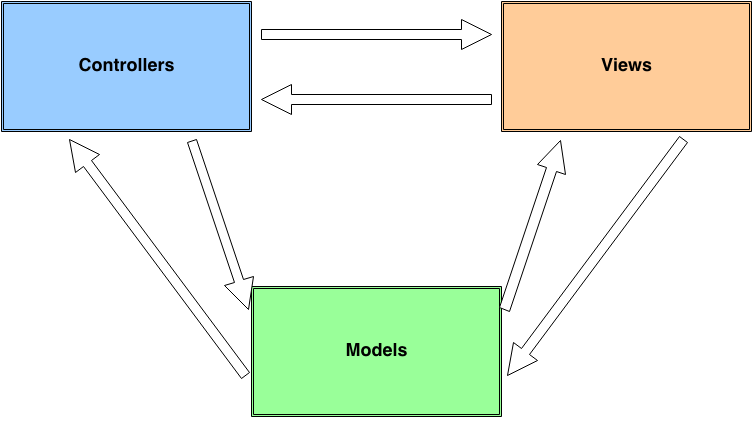
\includegraphics[height=3.5in]{figures/mvc.png}

    \caption[Model-View-Controller Architecture
    ]{A generic Model-View-Controller architecture.}

    \label{mvc}
\end{figure}

Controllers in AngularJS are stored as \emph{controllerName.js}. A controller in MVC is something that stores business logic that controls the web application. In AngularJS, any thing within the controller that is not a function will execute the moment that specific route is loaded. This includes any sort of models or JavaScript logic not wrapped in a function. Otherwise, the code within a function will not happen until that specific method is invoked. For example, all of the REST HTTP calls will happen right away when the controller is loaded.

Models in AngularJS are defined through the \$scope variable and are related to the variables that reside within the controller. The models are what contains data that is shown and also modified by the user. In the case of \projectName{}, these model data variables are usually data that \projectName{} queries from \ancor{}. An example of some of these data variables include instances, roles, and the \ancor{} version. AngularJS stores this data to make it easily accessible to the view.

Views in AngularJS are still in HTML, however developers are able to modify the DOM tags to contain Angular code that makes working with HTML a bit easier. The code segment in \ref{htmlcodefigure1} shows off an example of how AngularJS makes writing views easier. It is a code segment from \projectName{} where it builds a simple dropdown that contains all of the roles from \ancor{}. It gets the roles variable from the MainCtrl model and uses an AngularJS style for each to loop over all of the elements on roles to create a list of roles for the dropdown.

\begin{figure}[H]
  \begin{center}
    \renewcommand{\theFancyVerbLine}{
      \sffamily\textcolor[rgb]{0.5,0.5,0.5}{\scriptsize\arabic{FancyVerbLine}}}
    \begin{minted}[mathescape,
                   linenos,
                   numbersep=5pt,
                   gobble=2,
                   frame=lines,
                   framesep=2mm]{html}
    <ul class="dropdown-menu" role="menu" >
      <li ng-repeat="role in roles">
        <a ng-click="addNewRole(role)">
          {{role}}
        </a>
      </li>
    </ul>
    \end{minted}

  \end{center}
  \caption{AngularJS generating a dropdown menu.}
  \label{htmlcodefigure1}
\end{figure}

\subsection{Interacting with \ancor{} Through REST}

When \projectName{} needs to directly interact with \ancor{}, it communicates through a REST API, or Representational state transfer~\cite{DMatrix:Fielding:2000} API. Developed in 2000 by Roy Thomas Fielding, REST is a popular solution developers use when projects need to communicate to each other over HTTP.

By communicating over HTTP with REST, \ancor{} is able to expose a few functions that help outside users control the project. To start this process, you make an HTTP operation call to a specified URL. These operations are known as \emph{GET, POST, PUT,} and \emph{DELETE}. Since \ancor{} was designed to communicate to outside projects through REST, \projectName{} uses this API to send and receive data directly to \ancor{}. The following is a description of each component of the REST API basic functionalities with examples on how \projectName{} uses them.

\emph{GET} is a RESTful operation that when invoked, will return information depending on what endpoint has been queried. For example, if \projectName{} wants to get a detailed list of all the instances currently on \ancor{}, it can query the \emph{http://ancorIP/v1/instances} endpoint and get a json-formatted chunk of data that details all of the instances currently deployed.

\emph{POST} is a RESTful operation that allows information to be \emph{posted} to the remote server. This operation is often used when a website has form data that needs to be submitted to the remote server. In \projectName{}, \emph{POST} is used when a user is ready to submit a configuration file to deploy a new environment. In this case, we are not posted json formatted data to \ancor{}. In the header we put that the data is yaml format so \ancor{} knows what format to expect.

\emph{PUT} is a RESTful operation that implies that you are \emph{putting} or modifying a resource. This means you will replace whatever was there before with the new call. In \projectName{}'s case, this operation is used when we want to tell \ancor{} to commit the newly \emph{POSTED} environment.

\emph{DELETE} is a RESTful operation that will \emph{delete} a given resource depending on what endpoint is queried in \ancor{}. For example when a user wants to delete a given instance or an entire environment, they are able to make a \emph{DELETE} call to remove that given instance or environment.

\section{Use-Cases}
\label{makereference2.4}

In this section, I will describe the use-cases that this dashboard covers. These use-cases mirror the functionality of \ancorcli{}, but give a more visual interactive experience for the user instead of the terminal based experience \ancorcli{} gives.

\subsection{Viewing Instances}

The main use-case that this dashboard was developed for was seeing the state of instances from \ancor{}. This is also the main view of \projectName{} when you first visit the project in your browser. It displays how many instances \ancor{} currently has, as well as what current state each instance is in. If you scroll down, you can see the D3.js generated network graph. This graph displays the layout of \ancor{} and shows how each instance is related. This can be seen on figure \ref{mainInstanceView}. A closer look at the dynamically generated network graph can be seen in figure \ref{networkGraph}.

If a user wishes to see all of the instances of \ancor{} in more detail, they can scroll down to the table of instances near the bottom of the main page as seen in figure \ref{mainInstanceTableView}. In this case, the table shows the user the instance name, the interface it's on (an ip address), the current stage, and the planned stage. Clicking the more info button will display all of the relevant information that \ancor{} provides about each instance (figure \ref{modalInstanceView}). At the moment, there is no \ancor{} endpoint to query for any \emph{advanced} details, however there is a space left in case that feature is added in the future. The final column contains various operations that a user can perform on the instance as well.

If a user wants to search for something specific within the table, they are able to use the filter search box. As seen in figure \ref{instanceTableFilter}, when typing something in this box, the table will shrink down to match the search parameters.

\subsection{Viewing Tasks}

Visiting Tasks (figure \ref{tasksView}) will give you the state of all current tasks. They are sorted by tasks that were updated most recently and give a user an idea of what's currently happening on \ancor{}. For example, when a user deploys a new configuration, they are able to visit the tasks page to watch what tasks are currently in progress, what tasks have completed, or what tasks are suspended. They are also able to filter tasks if they are searching for something specific. The filter will work for any column in Tasks.

Like in the Main view, Tasks also has a filter search box to allow users to look through all Tasks. Typing anything in the search box will start the process of filtering through all of the Tasks data as seen in figure \ref{tasksFilter}.

\subsection{Deploying New Roles/Instances}

All roles can be discovered by selecting the dropdown link above the Instance overview table. Each element in the dropdown for adding a new role is the given role slug provided by \ancor{}. This dropdown can be seen in figure \ref{dropdownRoles}.

If a user wants to deploy a new role to \ancor{}, they can select one of the role slugs from the dropdown menu. \projectName{} will then make an HTTP POST call to \ancor{} with the selected role slug to deploy a new specified instance.

\subsection{Importing Configuration Specification Files}

\projectName{} provides an interactive method for deploying and importing configuration specifications. Visiting the Deploy endpoint for \projectName{} will load up the ACE embedded cloud editor (figure \ref{deployView}). This editor is fully featured and supports yaml syntax highlighting.

For the users convenience, \projectName{} provides two templates that can be inserted into the arml specification while they develop their configuration file (figure \ref{aceEditorSample}). The first one is the basic goal template that a user will have to make when starting a new configuration. The other template provided is a role template, which a user can insert after they have created a goal within the configuration specification. These templates provide some basic structure that a user can modify while developing their configuration specification.

If a user is confused on the structure of an configuration specification, they can select the help button on top of the ACE Editor (figure \ref{deployHelpView}), which will bring in a modal view explaining the structure as well as showing an example that they can use.

\subsection{Replacing and Deleting Instances}

For replacing an instance, \projectName{} provides a button on the main Instance table view that a user can select to perform the replace action (figure \ref{replaceDeleteInstance}). When the user selects replace, the view will invoke the replaceInstance method in the main controller with the given instance id. \projectName{} then does an HTTP POST call to \ancor{} against the id passed in from the view. At the moment, \ancor{} does not support replacing an instance. However the code is in place once this feature has been completed, and the only change required would be uncommenting out some code within the main controller.

Similar to replacement, \projectName{} provides a way for a user to delete instances as well. Selecting the delete button from the instance table list will invoke a function within the Main controller to do an HTTP DELETE call to \ancor{} with the provided id.

\subsection{Viewing Environments}

If a user would like to see if the current environment is locked, or if they are interested in the name of the current deployments environment, they can visit the Environments page of the dashboard (figure \ref{envView}). This view will also let the user know if the environment is currently locked. When an environment is locked, that means \ancor{} is currently working on a job and no other operations can occur.

\subsection{Deleting Environments}

When an \ancor{} user wants to completely remove an environment, they can visit the Environments page of the dashboard. This view provides a button that will completely remove the current deployment. After invoking this operation, the Tasks page will show the progress of removing the specific environment. The delete button will become disabled if the environment is locked.

\section{Interaction Diagrams}
\label{makereference2.5}

Interaction diagrams give a general overview of how a user might interact with the software the diagrams were based off of. In this section, I introduce \projectName{}s interaction diagrams based off of the use cases referenced in \ref{makereference2.4}.

In figure \ref{mainInterDiagram}, we have the interaction diagram for the Main, Env, and Task endpoints. The first event that happens is when a user visits one of the three endpoints on the dashboard. This will kick off a few HTTP GET calls which will interact with \ancor{}'s REST API. These HTTP GET calls are different depending on which endpoint we are looking at (this will be explained in the next chapter). Once the controller receives a response from \ancor{}, if successful, it will take the json data it received and store it in a model variable to be used for later. This model variable will also be displayed on the view for the user to see and interact with. If there are any updates made by the user through the view, those updates will also be made in the model because of AngularJS data binding. The views also have various functions that can interact with the controller. For example in the Main view, there are functions for creating and deleting instances. These functions are invoked from the controller, which then make the appropriate HTTP POST or HTTP DELETE calls to \ancor{}.

\begin{figure}[htb]%t=top, b=bottom, h=here

    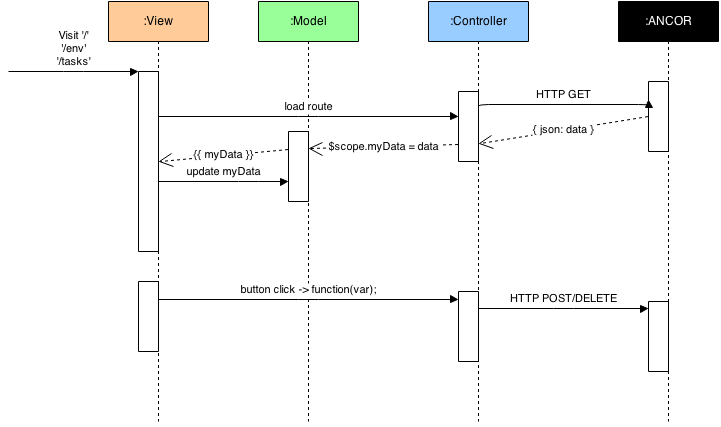
\includegraphics[height=3.5in]{figures/MainCtrl-Interaction-Diagram.png}

    \caption[Main, Env, and Task Interaction Diagram
    ]{Interaction diagram for Main, Environment, and Tasks endpoints.}

    \label{mainInterDiagram}
\end{figure}

In figure \ref{deployInterDiagram}, we have the interaction diagram for the Deploy endpoint. When this endpoint is first loaded up, it goes out and fetches environments from \ancor{}. This is so the user can be informed as to how many environments are currently deployed in \ancor{}. Currently, this is important because the dashboard only supports a single deployed environment. Next, the ACE editor is loaded up for the user to interact with. The user is able to have a full editor where they can write their configuration configuration file. As the user writes out their configuration, the View makes sure to update the model as to what is within ACE. Once the user clicks the deploy button, \projectName{} will take all of the text within the ACE Editor to send off to \ancor{}. It will first to an HTTP POST that contains the configuration data in yaml format. Once that call has been successful, it will do an HTTP PUT to let \ancor{} know to commit the changes and start the deployment.

\begin{figure}[htb]%t=top, b=bottom, h=here

    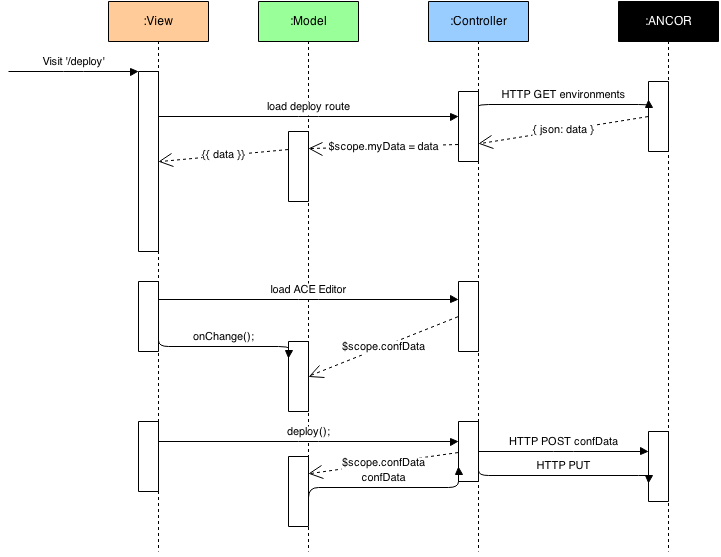
\includegraphics[height=4.5in]{figures/deploy-instance.png}

    \caption[Deploy Interaction Diagram
    ]{Interaction diagram for Deploy endpoint.}

    \label{deployInterDiagram}
\end{figure}
